\documentclass[9pt,twocolumn,twoside,lineno]{gsajnl}
% Use the documentclass option 'lineno' to view line numbers

\usepackage{epstopdf}

\articletype{inv} % article type
% {inv} Investigation
% {gs} Genomic Selection
% {goi} Genetics of Immunity
% {gos} Genetics of Sex
% {mp} Multiparental Populations

\runningtitle{GENETICS Journal Template on Overleaf} % For use in the footer
\runningauthor{FirstAuthorLastname \textit{et al.}}

\title{Act vs Rule Utilitarianism and Collisionavoidance Protocols of Autonomous Vehicles}

\author[1]{Jinghan Wang  z5286124}

\begin{abstract}
Compare and contrast act vs rule utilitarianism. How might their use to motivate collisionavoidance protocols for autonomous vehicles result in different protocols? Which of act and rule utilitarianism do you prefer for this purpose? Why? Justify your answer.
\end{abstract}

\keywords{2177}

\dates{\rec{20 09, 2022} \acc{10 10, 2022}}

\begin{document}

\maketitle
\thispagestyle{firststyle}
%\slugnote
%\firstpagefootnote
\vspace{-13pt}% Only used for adjusting extra space in the left column of the first page

\section{Introduction}
Spatial mobility has been a necessity for human beings since ancient times. Although the popularization of vehicles provides a lot of convenience, it also brings great negative effects. One of them is the transportation crashes, according to the survey, approximately $70\%$ to $90\%$ of transportation crashes is the result of human error \citep{dhillon2007human}. Making fewer mistakes and more responsive computers to handle the car instead of human has been proposed to solve the problem. As the practicability of allowing computer to ply public roads which provided by the development of chips and the tremendous improvement on computing power, increasingly more Internet company had committed to the research of self-driving.

There are six levels of autonomous driving in Figure \ref{fig:my_label}  which be defined by SAE J3016 according to the context of motor vehicles and their operation on roadways, ranging from SAE level 0 (no driving automation) to SAE level 5 (full driving automation). It also can be summarized into two categories. According to the figure, the main difference between two categories is level 0 - 2 required the driver makes the decision and the main decision of level 3 - 5 is made by the computer using the collisionavoidance protocol. From a programming perspective, going from level 0 to level 2, or from level 3 to level 5 isn't difficult which just requires refining different action by different scenarios. However, from level 2 to level 3, how to make the computer which can calculate to estimate the possible options and consequences in a split second do collision avoidance behaviours or distribute harms that conform to ethics, laws and are accepted by the society or the public under the pre-programmed collisionavoidance protocols is the most difficult and is also the key to evolving from an assisted driving system to an autonomous driving system.

Nowadays, there are many ethical foundations for the mainstream computer collisionavoidance protocols, and the protocol based on utilitarianism is one of them that has attracted much attention.  In this paper, will focus on two kinds of utilitarianism, act utilitarianism and rule utilitarianism, as well as the different results of using them to motivate collisionavoidance protocols for autonomous vehicles.
\begin{figure}
    \centering
    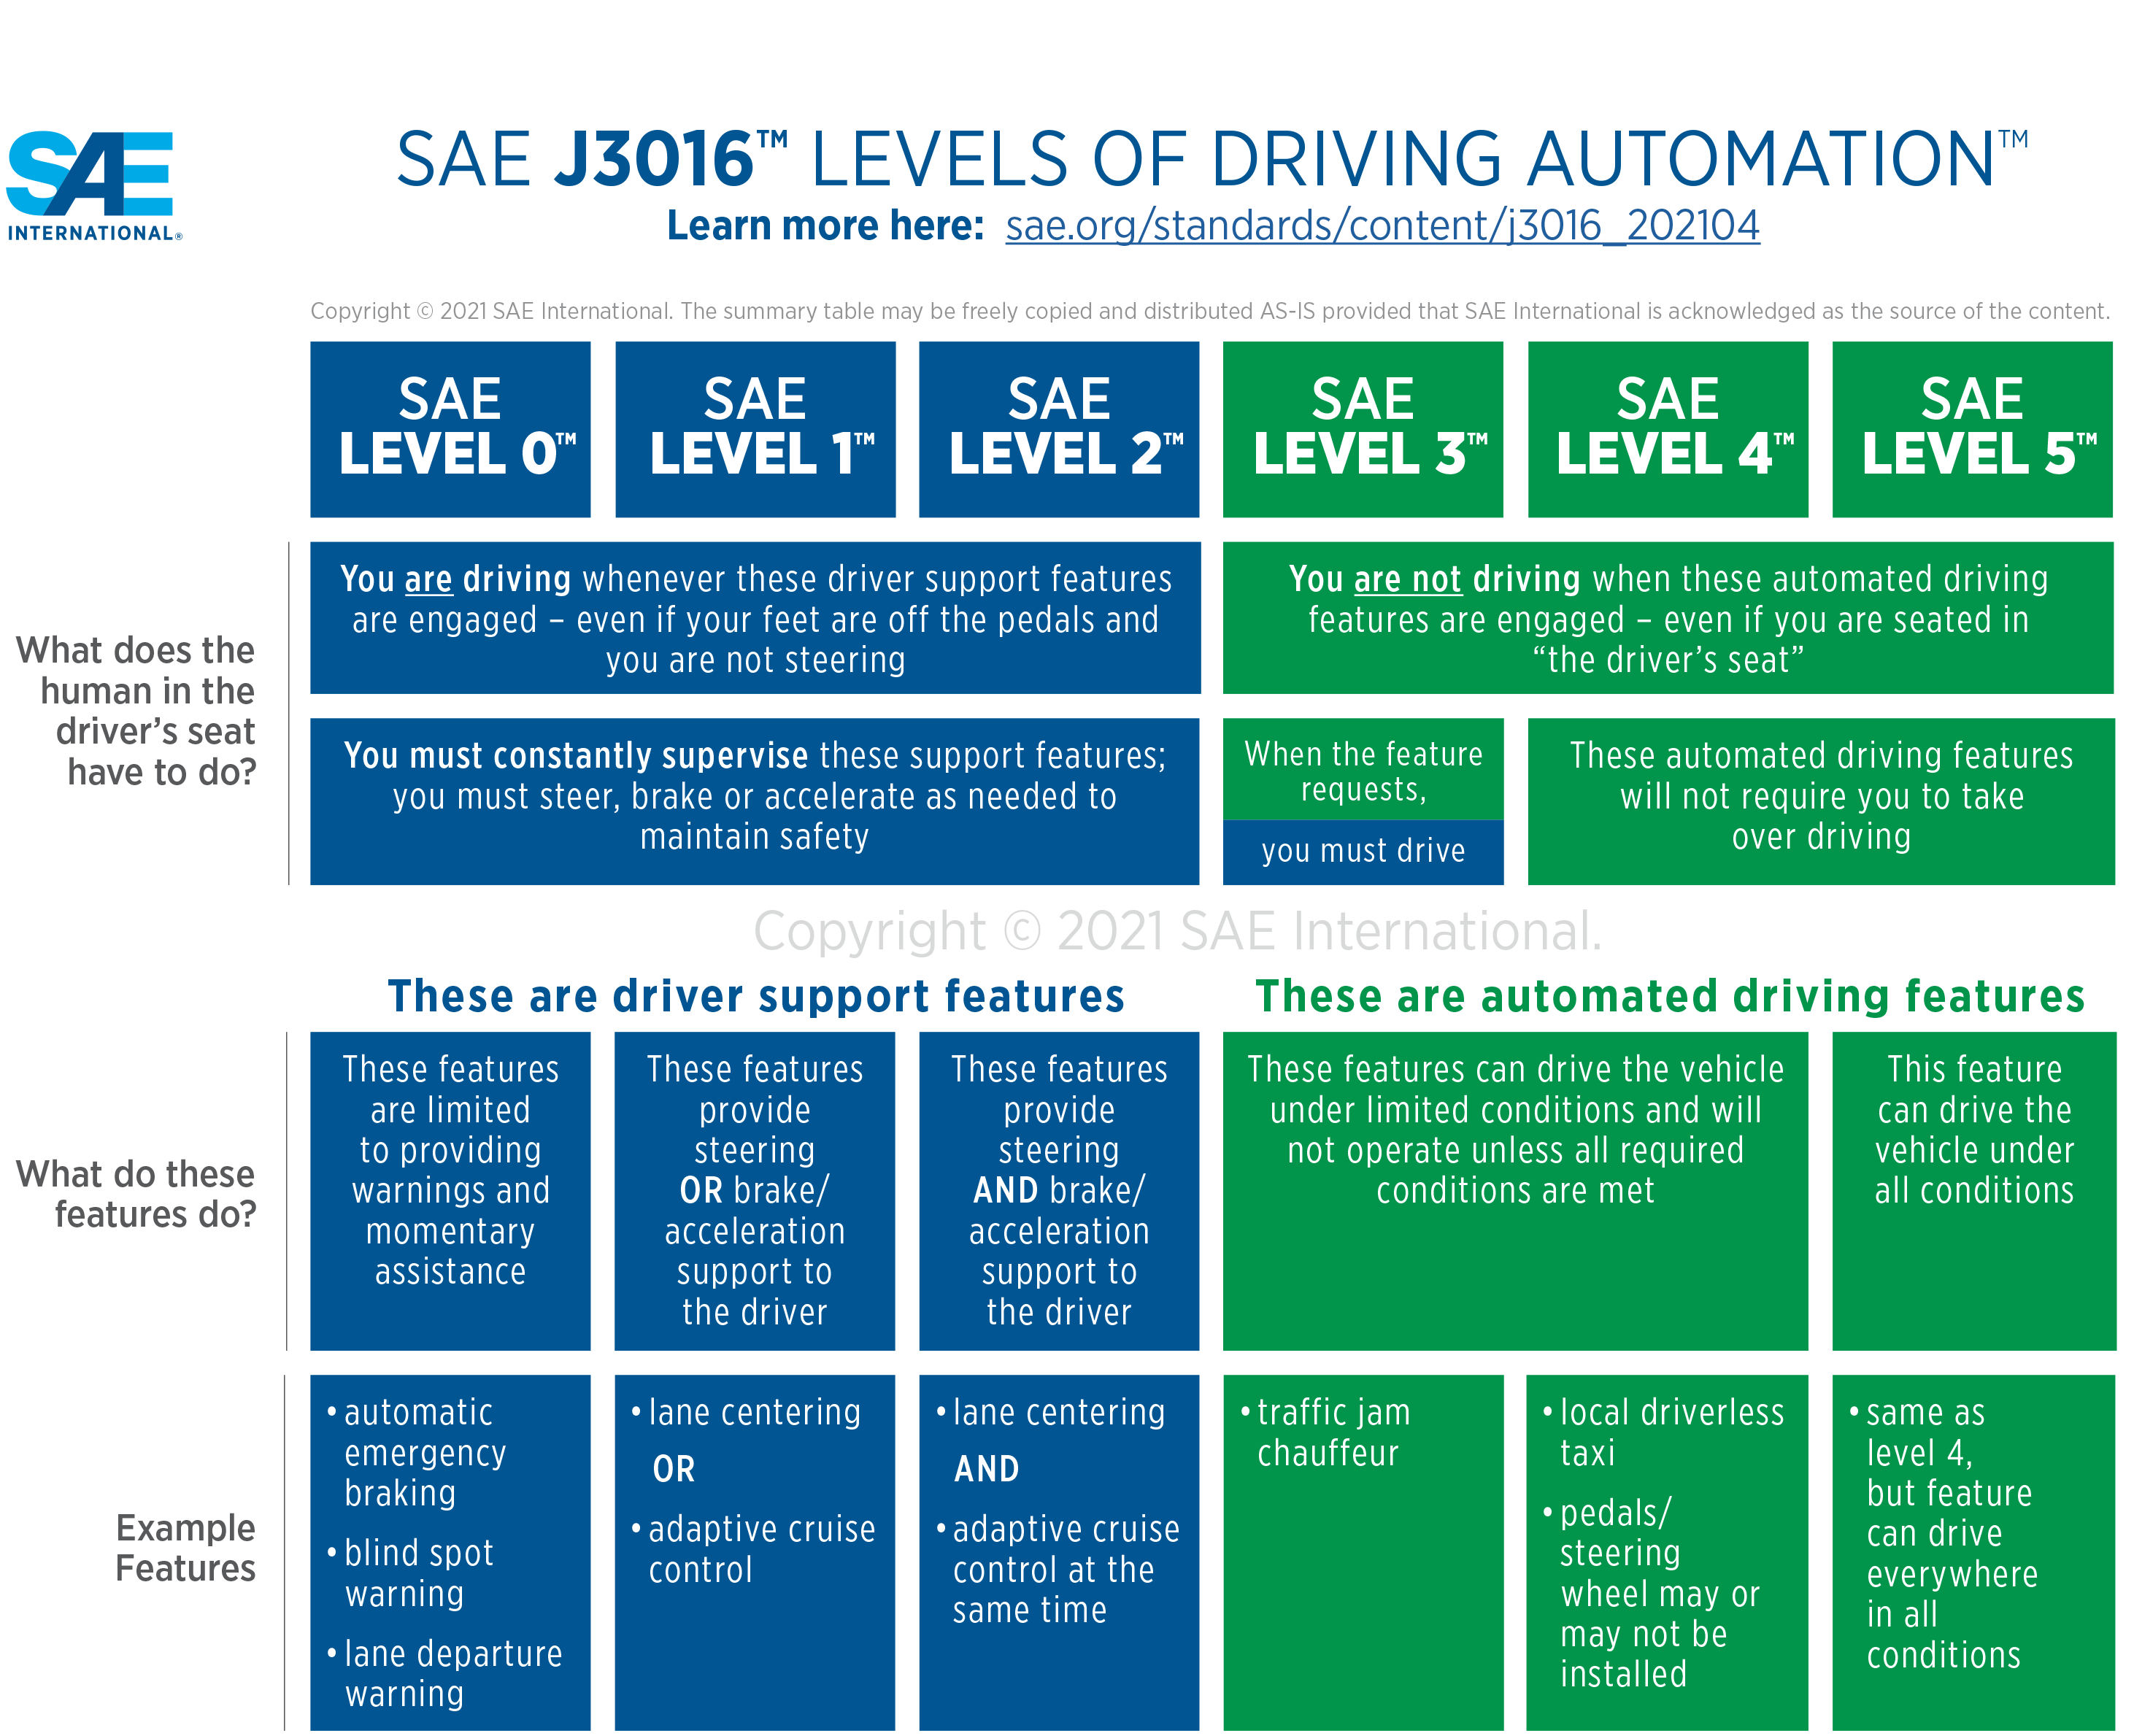
\includegraphics[width=\linewidth]{j3016graphic_2021.png}
    \caption{SAE J3016™ Levels of driving automation \citep{SAE2021}}
    \label{fig:my_label}
\end{figure}



\section{Utilitarianism}
Utilitarianism is a consequentialism ethical theory found by the British philosopher Jeremy Bentham in the late 18th century, which holds that the correct behaviour is to maximize the benefit and prefer to avoid pain as much as possible. 
\subsection{Act Utilitarianism}
Act Utilitarianism holds that an action is correct if and only if it produces the best possible result from everything that might be involved. It compares it to an math algorithm that any action or decision can be abstract as the sum of all the pleasures it produces minus the pain of all the human involved.   The larger the difference result, the more inclined to achieve.   So act utilitarian needs to consider the options available when makes a decision, analyse and choose the option which one brings more happiness and less pain to all involve.   This theory is conducive to the maximization of happiness, it pursues fairness, everyone regardless of gender, age, social class, even any creature has the same happiness weight during the calculating.

However, It is the problem and unfair with this theory that since the Act Utilitarianism is consequentialism, it does not judge the nature or the process of any action, the right or wrong of any action is only related to whether it can achieve the maximum happiness,  it acquiesces in achieving the happiness and happiness of the majority at the cost of a few unhappy and even miserable human.  Even the behaviour of slavery, framing innocence to make peace and so on which is reviled by morality, is desirable.  In other ways it is impractical, when a human needs to calculate a lot of possibilities and results before making every decision, this thing itself is boring, and even affects the work efficiency and life states, which is not conducive to human happiness.
\subsection{Rule Utilitarianism}
Rule utilitarianism is another form of utilitarianism, which emphasizes that it is only right to act in accordance with the principle of maximizing the good, in other words, it is correct or will not be problematic that act in accordance with a set of ideal moral rules. In terms of ideal moral rules that need to be observed by all human, rule utilitarians expound that first is fair, ideal moral rules are universal and apply to all humans. The second is the maximization of utility, which can bring the best consequences to people. Construct two opposite worlds through imagination, one follows certain rules and the other does not. Compare which of the two worlds will be happier, then the rules that the world follows should be the ideal moral rules.

Because of the moral rule, the extreme case of rule utilitarianism, slavery, framing to keep the peace will be avoided as it's inherently wrong with the principle and disallowed regardless of the consequences. However, the judgment of many behaviours is not a binary problem, it has two sides such as lies are not advisable, but white lies for the greater happiness of others without harming the other's interest should be encouraged. The difference between lies in different scenarios and different intentions. It is biased to judge the good or bad of an action directly by imagining two worlds. Assume a behaviour through torture to prevent terrorism, torture is not approved by the rule utilitarian as the world full of torture as absolutely no torture of social happiness. However, in order to satisfy the moral rules, brought the disaster to more people, it seems to become a rule worship without considering the actual situation.

\subsection{The difference between Act and Rule Utilitarianism}
Compare act utilitarianism to rule utilitarianism, for act utilitarianism is only concerned with outcomes which doesn't care about what's right or wrong in the process. In contrast, rule utilitarianism is similar to deontology that the world will be happier only if human needs to follow some moral rules. They ignore the possibility which may lead by the complex society, regardless of the occasion and situation to judge an action to be right or wrong and then requires everyone to follow this rule under all circumstances. Although both aim to maximize happiness, both are idealistic.


\section{Utilitarianism and Collisionavoidance protocols}
The traffic scenario encountered by self-driving vehicles can be likened to the famous thought experiment, the trolley problem \citep{foot1967problem, judith1985trolley}, where suppose the driver of a runaway trolley can only switch from one track to another, On the straight track ahead, there are five persons. Simultaneously, one person is on another track, as long as the trolley enters the track, all the people on track will die. Should the driver steer for the less occupied track?

\subsection{Collisionavoidance protocols motivate by Act Utilitarianism} 
For act utilitarianism, it mainly focuses on maximizing human happiness, which is mainly reflected in the minimum casualties in this collisionavoidance protocols.   So, with that goal in mind, in the trolley problem, it will choose to change lanes to save more people at the expense of one person.   Under the collisionavoidance protocols inspired by act utilitarianism, every human or creature that may be involved in the threat is fair, and every person's life has the same weight in the calculation and will not be affected by age, gender, status, and wealth.   Different from the trolley problem, in the real accident, there are different degrees of damage, so the computer needs to calculate the possible protection or additional damage caused by the items and equipment carried by all humans.   Death has the lowest weight, and injury is given a higher weight according to the lighter possible injury.   The computer needs to calculate all the possibilities and compare all the possibilities leading to the least number of casualties, the probability of the least number of casualties, the highest weight of the behaviour to implement, as to minimize the accident to all the personnel brought harm.   Theoretically,this is in line with society's expectations for autonomous driving technology theoretically.

However, there are still problems with this ethical collisionavoidance protocols.  Because injury and death have different degrees of weight, self-driving vehicles are more likely to hit drivers who obey traffic rules and take protective measures, and avoid drivers who do not take protective measures, because the latter is less likely to be killed or injured.  Whether this behaviour is penalized for virtue and encourages non-virtuous behaviour because carrying less protective gear will make the computer more inclined to dodge.  Obviously, this is unfair.  When an accident assumes that there are perpetrators and innocent people, it is not fair and socially acceptable to let innocent people bear the consequences that may cost their lives for the perpetrator's behavior in order to minimize casualties.

\subsection{Collisionavoidance protocols motivate by Rule Utilitarianism}
For the collisionavoidance protocols under rule utilitarianism, it requires the machine to make a choice under the judgment of whether all human involved in the accident follow the moral rules. If the human who caused the accident violates the moral rules, the machine should lower his or her weight and higher the weight for innocent human who might be affected. So making the rule will be the key to design Collisionavoidance protocols. First, the existing traffic laws and regulations are worth following because of enough authority and more suitable for the society. Suppose that when traffic accidents are caused by human who do not obey traffic rules, it is inclined to protect the innocent, at the expense of those who do not obey traffic rules. In addition, It also requires a series of rules when it has to weigh innocent people so that the computer can judge the more favourable option. By assuming several worlds, protect which kinds of innocent human will be more beneficial to human development, then this human will have higher weight than others. Suppose that when the choice is between an innocent pregnant woman and an innocent man, because protecting the pregnant woman is more beneficial to human development, then the pregnant woman has a higher weight in the calculation. Therefore, based on the collisionavoidance protocols under rule utilitarianism in the trolley problem is that judge five humans' behaviour, if they are violating the rules, cannot be at the expense of a person to in order to save five people. If they are not violated, based on their age, physical condition, contribution to the society and other rules to determine whether the trolley should be turned.

It seems that this collisionavoidance protocols is better. It will not let innocent people take the place of perpetrators to be punished to a large extent to avoid greater disasters.    It also achieves the sustainable development of society by protecting the safety of people who may provide greater value to the society. But because of this, it is extremely unfair, for example, the unintelligent seem to be defined from birth as more deserving of sacrifice to preserve the intelligent in order to achieve better social development than the intelligent. The other question is that how to set the priority of age, gender, possible contribution to society and so on.    Under this kind of protocols, each human is forced to be assigned a different class according to the rules of age, gender, intelligence, and possible contribution to society, etc., The act of classifying people according to their status is essentially as bad as slavery behaviour and is also not socially acceptable.


\section{Discussion}
In my opinion, the collisionavoidance protocol under act utilitarianism is the better choice. First, from minimizing accident casualties, the sooner the concise calculation, the more conducive to avoid greater disaster, motivate collisionavoidance protocols under act utilitarianism only need calculate possible casualties to act by best possibility.   The rule utilitarian needs to search a huge mass of data, this not only waste precious time, also need real-time connection network and keep the network unobstructed at the same time, in order to achieve anytime anywhere query.   In addition, collisionavoidance protocol under rule utilitarianism, due to the different cultures will produce different values, the moral rules, or each character involving the comparison of the weight cannot in line, which may lead to different judgments about the accident.  Compare to act utilitarianism, since the goal is to minimize casualties, the agreements designed by different companies will be similar.  When multiple vehicles are designed for similar collisionavoidance protocols, it will be easier to reach the same judgment, thus reducing the possibility of casualties.  What is more, collisionavoidance protocols under act utilitarianism are easier for programmers to write and covering the possibility of more accidents, the protocol under the rule utilitarianism, needs to consider more scenarios, and is prone to more negligence and error.


\section{Conclusion}
Therefore, the main reason why no autonomous vehicle for any brand will be able to break SAE level 3 in the short term is that there is no crash-avoidance protocol for everyone. Therefore, the complete SAE level 5 fully autonomous vehicle is impossible to implement in the short term. For SAE level 2 to SAE level 3 crossing in the short term, the collisionavoidance protocols of the vehicle may not be required to fully make decisions similar to the trolley problem, but it is more necessary to predict and avoid accidents in advance.    It also needs the support of the corresponding environment.\nocite{*}
\bibliography{References}

\end{document} 